\begin{frame}{冬の 10 hPa が東風なのは\\アリューシャン高気圧の西縁だから}{考察}
  \begin{columns}[T]
    \begin{column}{0.44\textwidth}
      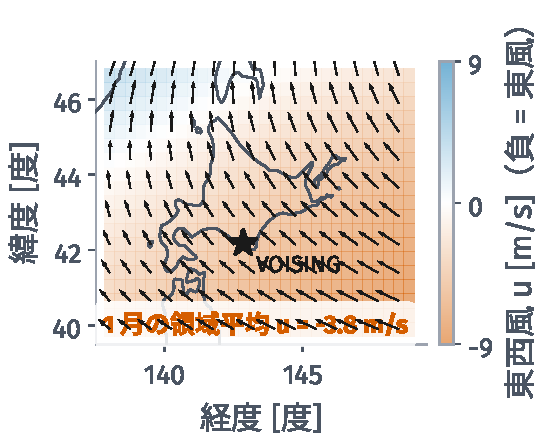
\includegraphics[width=\linewidth,height=124pt,keepaspectratio]{S_map_10hpa_jan.pdf}
    \end{column}
    \begin{column}{0.54\textwidth}
      {\centering
      \begin{tikzpicture}[x=1mm,y=1mm,>={Latex[length=2mm,width=1.6mm]}]
        \fill[wcGrey] (-33,-9) rectangle (33,9);
        \node[font=\fontsize{8.5}{10}\selectfont,text=wcSecondary,anchor=north west] at (-32.5,8.5) {北太平洋の成層圏（10 hPa、真冬）};
        \draw[wcBlue,line width=1.2pt,->] (15,-2.5) ++(150:10 and 4.8) arc (150:-160:10 and 4.8);
        \node[font=\mediumfont\fontsize{8.5}{10}\selectfont,text=wcBlue,align=center] at (15,-2.5) {アリューシャン\\高気圧};
        \fill[wcMuted] (-19,-3.5) ellipse (2 and 3.6);
        \node[font=\fontsize{8.5}{10}\selectfont,text=wcSecondary,anchor=east] at (-21.5,-3.5) {日本};
        \draw[wcOrange,line width=1.5pt,->] (-4,-2.5) -- (-15,-2.5);
        \node[font=\mediumfont\fontsize{9}{10.5}\selectfont,text=wcOrange,anchor=north] at (-9.5,-3.6) {東風};
      \end{tikzpicture}\par}
      \vskip 0.8mm
      \begin{itemize}\itemsep 0.4mm
        \item 帯状平均では冬の中緯度成層圏は\kw{西風}
        \item 1 月の 10 hPa は\warn{東風 $-3.8$ m/s}、各年とも
        \item 高気圧の西縁にあたる \src{Harvey+96}
        \item 帯状平均を扇形の領域に当てはめない
      \end{itemize}
    \end{column}
  \end{columns}
\end{frame}
